% d03-tikz: TikZ (xetex driver): paths, fills, dashes, arrows, text nodes, transforms and rotation, opacity, axial and radial shading, clipping, a tiling pattern
\documentclass{article}
\usepackage{fontspec}
\usepackage{tikz}
\usetikzlibrary{arrows.meta,patterns}
\begin{document}
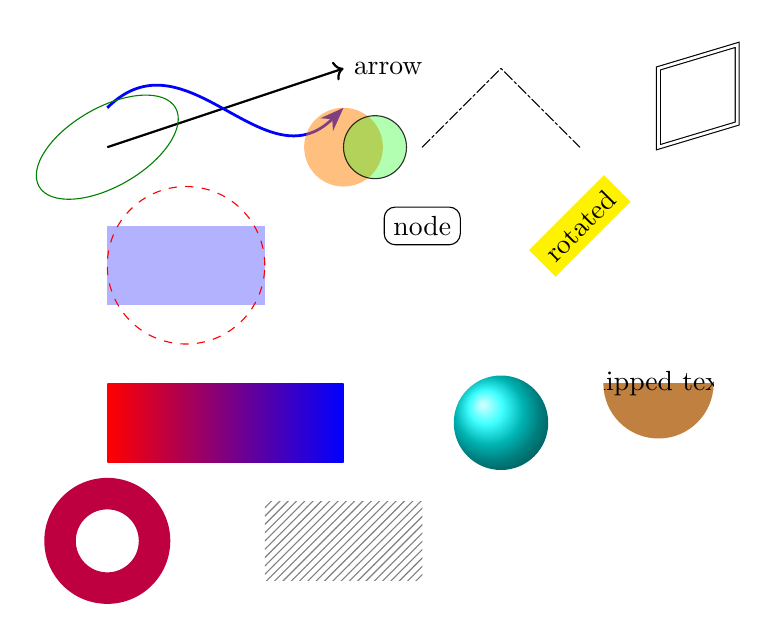
\begin{tikzpicture}
\draw[thick,->] (0,0) -- (3,1) node[right]{arrow};
\draw[-{Stealth[length=3mm]},blue,line width=1pt] (0,0.5) .. controls (1,1.5) and (2,-0.5) .. (3,0.5);
\fill[blue!30] (0,-1) rectangle (2,-2);
\draw[red,dashed] (1,-1.5) circle (1);
\draw[dash pattern=on 4pt off 1pt on 1pt off 1pt,line cap=round,line join=round] (4,0) -- (5,1) -- (6,0);
\node[draw,rounded corners] at (4,-1) {node};
\node[rotate=45,fill=yellow] at (6,-1) {rotated};
\draw[rotate=30,green!50!black] (0,0) ellipse (1 and 0.5);
\begin{scope}[xshift=7cm,scale=0.5,yslant=0.3]
  \draw[double,double distance=1pt] (0,0) rectangle (2,2);
\end{scope}
\fill[orange,opacity=0.5] (3,0) circle (0.5);
\fill[green,fill opacity=0.3,draw=black,draw opacity=0.8] (3.4,0) circle (0.4);
\fill[even odd rule,purple] (0,-5) circle (0.8) (0,-5) circle (0.4);
\shade[left color=red,right color=blue] (0,-3) rectangle (3,-4);
\shade[ball color=cyan] (5,-3.5) circle (0.6);
\begin{scope}
  \clip (7,-3) circle (0.7);
  \fill[brown] (6,-4) rectangle (8,-3);
  \node at (7,-3) {clipped text};
\end{scope}
\fill[pattern=north east lines,pattern color=gray] (2,-5.5) rectangle (4,-4.5);
\end{tikzpicture}
\end{document}
